\section{Equivalence of Hardware and Software Netlist}
%
The consistency between two designs can be established in several ways. 
For example, few common notion of consistency criteria are \emph{behavioral}, 
\emph{cycle-accurate}, \emph{non-cycle accurate} or \emph{functional}
consistency.  The consistency between a reference model and an implementation
model is performed through systematic equivalence checking~\cite{}.  Equivalence
checking between a timed and untimed model is a hard
problem~\cite{}.  Sequential equivalence checking techniques are used to check 
the equivalence between an asynchronous event driven semantics of C and synchronous 
clock driven semantics of Verilog~\cite{}.


%%%%%%%%%%%%%%%%%% CYCLE ACCURATE EQUIVALENCE %%%%%%%%%%%%%%%%%
Two designs are said to be \emph{cycle-accurate-equivalent}~\cite{cycle} \rmcmt{more
reference} if they produce the same output using the same number of clock cycles.   

%%%%%%%%%%%%%%%%%% NON-CYCLE ACCURATE EQUIVALENCE %%%%%%%%%%%%%%%%%
Whereas, two designs are \emph{not cycle-accurate-equivalent}~\cite{cycle} if they require 
different cycles to perform the same computation. For example, consider two circuits
implementing the Euclid's algorithm to compute Greatest Common Divisor (GCD),
where Circuit A uses two subtractors and Circuit B uses one subtractor.  In this
case, Circuit B requires more cycle than Circuit A to compute the GCD. Thus,
they are functional-equivalent but not cycle-accurate-equivalent. However,
Circuit A and Circuit B can be made cycle-accurate-equivalent by making Circuit
A to stutter for few cycles until Circuit B finishes its slower operation.  This
may require some additional logic in Circuit A to determine the condition for 
stuttering.  


In this paper, we assume a restricted notion of cycle-accurate-equivalence
between a hardware RTL and a software netlist to establish their consistency.  
We describe this next. 
%%%%%%%%%%%%%%%%%% RESTRICTED CYCLE ACCURATE EQUIVALENCE %%%%%%%%%%%%%%%%%
\rmcmt{Observability Preserving Equivalence}
\para{Cycle-accurate-Property-Equivalence}
%
Recall that a software netlist is derived from a hardware circuit for the
purposes of formal verification.  To this end, the design properties 
(temporal or non-temporal) over RTL signals that captures hardware behaviors 
are translated into assertions over the corresponding software variables and 
checked for consistency against the software
netlist model.  Thus, our notion of cycle-accurate-equivalence is 
limited to the signals that are observable in the property.  
We call this equivalence criteria \emph{cycle-accurate property-equivalence}.  
Intuitively, this means that the state of latches and wires 
present in the property match with the corresponding variables in software 
netlist model at some designated clock cycle.  The effect of a clock cycle 
in the software netlist model is simulated through an invocation of the top 
level procedure which corresponds to the top level module of the hardware circuit. 
\rmcmt{Note that a software netlist is synthesized from a hardware
RTL for the purposes of formal verification, just like a bit-level netlist or
word-level netlist are synthesized from an RTL. So, the proposed consistency 
criteria is sufficient for this purpose.  Techniques for translation
validation~\cite{} that check the consistency between a RTL and software 
is a different problem and beyond the scope of this work.}
%
\begin{definition} (Cycle-accurate-Property-Equivalent) 
  Two designs $C_1$ and $C_2$ are \emph{Cycle-accurate-Property-Equivalent} with
  respect to a property $P$ if the following conditions holds true. 
  \begin{enumerate}
    \item For a non-temporal property $P$, the result of analysis of $P$ must
      match in $C1$ and $C2$ at every clock cycle.  
   \item For a temporal property $P$, the result of analysis of $P$ must 
     match in $C_1$ and $C_2$ at some \emph{designated} clock cycle.  Such
      designated clock cycle are determined from the temporal operator used in $P$. 
  \end{enumerate}
\end{definition}
%
Two designs $C_1$ and $C_2$ are \emph{not} cycle-accurate property equivalent 
with respect to a non-temporal property $P$ if there exists a clock cycle where 
the result of analysis of $P$ does not match.  Intuitively, this means that 
there exists some latches or wires and a cycle $N$ where the observable signals in $P$ 
does not match in $C_1$ and $C_2$, resulting in inconsistent result of anaysis of $P$. 
%
Whereas, two designs $C_1$ and $C_2$ are \emph{not} cycle-accurate property equivalent 
with respect to a temporal property $P$ if there exists a \emph{designated} clock cycle 
where the result of analysis of $P$ does not match. 



%%%%%%%%%%%%%%%%%% EXAMPLE %%%%%%%%%%%%%%%%%
\begin{example}
%
Figure~\ref{figure:prop1} gives an example of a Verilog RTL (in left) and 
the corresponding software netlist in C (in right) that is 
cycle-accurate-property-equivalent but \emph{not} cycle-accurate-equivalent 
with respect to a temporal property (marked in red).  The property of Verilog 
is specified in SystemVerilog Assertion (SVA)~\cite{SVA} language.  
The equivalent assertion in software netlist is shown in the right (marked in red).  

We explain the condition for which the models are \emph{not}
cycle-accurate-equivalent.  Suppose $in=1$ at clock cycle $i$. 
Then, the state of the latch $out3$ is not consistent in 
Verilog and C at cycle $i$.  This is due to the fact that 
the value of $out3$ \emph{stabilizes} one cycle after the 
input $in=1$ was set, that is, $out3$ is stabilized in cycle $i+1$.  
This behavior is formally captured 
in SVA using the constraint \texttt{(in==1 |-> \#\#1 out3)}.  The SVA 
specifies that latch $out3$ is high exactly one cycle after $in$ was high.  

\rmcmt{state equivalent condition}


Both the models are \emph{safe} in this case, that is, the property 
holds true in both models.  The property is proven equivalent for 
unbounded cycles using a hardware model checker and a software verifier.  
Thus, a software netlist must be cycle-accurate-property-equivalent to a
hardware RTL for the purposes of formal verification. 

\end{example}
%


%Thus, the example in Figure~\ref{figure:prop1} demonstrate that the designs 
%are cycle-accurate-property-equivalent but not cycle-accurate-equivalent.
%
\begin{figure}[htbp]
\scriptsize
\begin{tabular}{l|l}
\hline
Verilog & C \\
\hline
\begin{lstlisting}[mathescape=true,language=Verilog,style=base]
module M(clk, in, 
     out1, out2, out3);
input clk,in;
output reg out1, 
     out2, out3;
wire t1;

initial begin
out1=0; 
out2=0;out3=0;
end

assign t1=out1;

always @(in) begin
out1 <= in;
end

always@(t1) begin
out2 <= t1;
end

always@(posedge clk) 
begin
out3 <= out2;
end
endmodule

module main(clk);
input clk;
wire in,out1,
     out2,out3;
M m1(clk,in,out1,out2,out3);
~assert property ~
 ~(out2==1 |-> ##1 out3);~
endmodule
\end{lstlisting}
&
\begin{lstlisting}[mathescape=true,language=C,style=base]
struct state_M {
 bool out1, out2, out3; 
};
struct state_M sM;

void initial() {
 sM.out1=0; sM.out2=0; 
 sM.out3=0;
}

void M(bool clk, bool in, 
 bool *out1, bool *out2, 
 bool *out3) {
  bool t1;
  sM.out3=sM.out2;
  sM.out1=in;
  t1=sM.out1;
  sM.out2=t1;
  // update output  
  *out1=sM.out1;
  *out2=sM.out3;
  *out3=sM.out3;
}
 
int main()
{
 bool clk,in,
 out1,out2,out3;
 initial();
 M(clk,in,out1,
 out2,out3);
 ~if(sM.out2) {~
  ~M(clk,in1,in2,~
  ~out1,out2,out3);~
  ~assert(sM.out3);~
 ~}~
}
\end{lstlisting}
\\
\hline
\end{tabular}
\caption{Cycle-accurate Property Equivalence}
\label{figure:prop1}
\end{figure}
%
\begin{figure}[t]
\begin{center}
  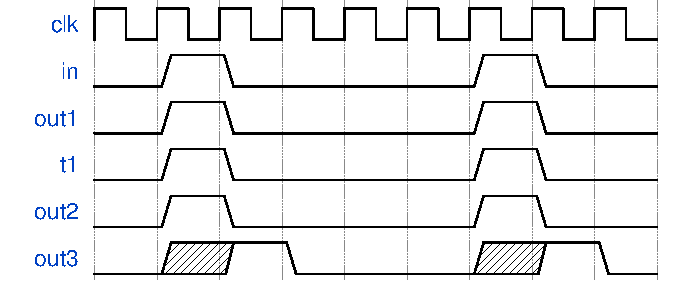
\includegraphics[width=\columnwidth]{figures/wavedrom.pdf}%
  \caption{Waveform view showing behavior of RTL design in
  Figure~\ref{figure:prop1}} 
\label{fig:waveform}
\end{center}
\end{figure}


%%%%%%%%%%%%%%%%%% LTL Semantics to C %%%%%%%%%%%%%%%%%
%\para{LTL to C program}
%
Linear Temporal Logic (LTL)~\cite{} is a modal logic that is commonly used to
reason about a hardware transition system.  The modalities in LTL refers to
temporal operators like $G$ (global), $F$ (eventaul), $X$ (next) and $U$
(until).  An LTL formula may contain propositional symbols, boolean or temporal
operators.  We skip the details of LTL since this is standard. 

The translation of LTL to a \emph{Buchi Automaton}
(BA) is an well-known technique~\cite{Gastin:2001, SomenziB00} and has been
sucessfully used for LTL model checking such as Spin model checker~\cite{spin}.   
Further, a buchi automaton can be modeled using a C program that simply encodes
the state transition relation of BA.  Figure~\ref{prop} gives an example of LTL
and the corresponding assertion in $\mathcal{SN}$.  Note that the next operator
(X) in LTL is modeled by invoking the top level procedure
$M(clk,in1,in2,out1,out2,out3)$ in $\mathcal{SN}$ which also 
corresponds to the top level module of the hardware circuit. 
%
\begin{figure}[t]
\scriptsize  
\centering
\begin{tabular}{|l|l|}
\hline
 Buchi Automaton & Assertion in $\mathcal{SN}$ \\
\hline
\begin{minipage}{3.5cm}
\scalebox{.5}{\import{figures/}{property.pspdftex}}
\end{minipage}
&
\begin{lstlisting}[mathescape=true,language=C]
if(sM.out2) {
  M(clk,in1,in2,out1,out2,out3);
  assert(sM.out3);
}
\end{lstlisting}
\\
\hline
\end{tabular}
\caption{LTL and its corresponding C Assertion}
\label{prop}
\end{figure}
%
The goal of this translation is to perform formal property verification 
of the software netlist model $\mathcal{SN}$ against the assertion 
expressed over the variables of $\mathcal{SN}$.  
%
While we do not have a formal proof of correctness, experiments have shown that for 
property verification, valid safety properties are proven to be $k$-inductive for 
the same unwind depth $k$ in the hardware and software netlist models.  Conversely, 
for unsafe designs, the bug is found in the same unwind depth for both the models.
